% Copyright 2004 by Till Tantau <tantau@users.sourceforge.net>.
%
% In principle, this file can be redistributed and/or modified under
% the terms of the GNU Public License, version 2.
%
% However, this file is supposed to be a template to be modified
% for your own needs. For this reason, if you use this file as a
% template and not specifically distribute it as part of a another
% package/program, I grant the extra permission to freely copy and
% modify this file as you see fit and even to delete this copyright
% notice. 

\documentclass{beamer}
% Replace the \documentclass declaration above
% with the following two lines to typeset your 
% lecture notes as a handout:
%\documentclass{article}
%\usepackage{beamerarticle}
\setbeamertemplate{navigation symbols}{\insertlogo}
\usepackage[orientation=landscape,size=custom,width=16,height=10,scale=0.5,debug]{beamerposter} 


% There are many different themes available for Beamer. A comprehensive
% list with examples is given here:
% http://deic.uab.es/~iblanes/beamer_gallery/index_by_theme.html
% You can uncomment the themes below if you would like to use a different
% one:
%\usetheme{AnnArbor}
%\usetheme{Antibes}
%\usetheme{Bergen}
%\usetheme{Berkeley}
%\usetheme{Berlin}
%\usetheme{Boadilla}
%\usetheme{boxes}
%\usetheme{CambridgeUS}
%\usetheme{Copenhagen}
%\usetheme{Darmstadt}
%\usetheme{default}
%\usetheme{Frankfurt}
%\usetheme{seahorse}
\usetheme{Goettingen} % This is the best
%\usetheme{Hannover}
%\usetheme{Ilmenau}
%\usetheme{JuanLesPins}
%\usetheme{Luebeck}
%\usetheme{Madrid}
%\usetheme{Malmoe}
%\usetheme{Marburg} % This one is good too
%\usetheme{Montpellier}
%\usetheme{PaloAlto}
%\usetheme{Pittsburgh}
%\usetheme{Rochester}
%\usetheme{Singapore}
%\usetheme{Szeged}
%\usetheme{Warsaw}
\usepackage{tikz}
\usetikzlibrary{tikzmark}
\usepackage{graphicx}
\usepackage{amsmath}
\usepackage{amssymb}
\usepackage{amsthm}
\usepackage{lipsum}
\usepackage{amsfonts}
\usepackage{fancyvrb}	 
\usepackage{forest}
\usepackage{multirow}
\usepackage{nicefrac}
\usepackage{multicol}
\usepackage{booktabs}
\usepackage{listings}
\usepackage{color}
\usepackage{wasysym}
\usepackage{xspace}
\usepackage{wrapfig}
\usepackage{todonotes} % for missing figure
\usepackage[utf8]{inputenc}
\usepackage[scaled = 0.95]{helvet}
\usepackage{hyperref}
\hypersetup{
	colorlinks = TRUE,
	urlcolor = blue,
	linkcolor= blue
}
%\usepackage{kpfonts}
%\usefonttheme{professionalfonts} % using non standard fonts for beamer
%\usefonttheme{serif} % default family is serif
\definecolor{mygreen}{rgb}{0,0.6,0}
\definecolor{mygray}{rgb}{0.5,0.5,0.5}
\definecolor{mymauve}{rgb}{0.58,0,0.82}

\lstset{ %
	backgroundcolor=\color{white},   % choose the background color; you must add \usepackage{color} or \usepackage{xcolor}
	basicstyle=\footnotesize,        % the size of the fonts that are used for the code
	breakatwhitespace=false,         % sets if automatic breaks should only happen at whitespace
	breaklines=true,                 % sets automatic line breaking
	captionpos=b,                    % sets the caption-position to bottom
	commentstyle=\color{mygreen},    % comment style
	deletekeywords={...},            % if you want to delete keywords from the given language
	escapeinside={\%*}{*)},          % if you want to add LaTeX within your code
	extendedchars=true,              % lets you use non-ASCII characters; for 8-bits encodings only, does not work with UTF-8
	frame=single,	                   % adds a frame around the code
	keepspaces=true,                 % keeps spaces in text, useful for keeping indentation of code (possibly needs columns=flexible)
	keywordstyle=\color{blue},       % keyword style
	language={},                 % the language of the code
	otherkeywords={*,...},            % if you want to add more keywords to the set
	numbers=left,                    % where to put the line-numbers; possible values are (none, left, right)
	numbersep=5pt,                   % how far the line-numbers are from the code
	numberstyle=\tiny\color{mygray}, % the style that is used for the line-numbers
	rulecolor=\color{black},         % if not set, the frame-color may be changed on line-breaks within not-black text (e.g. comments (green here))
	showspaces=false,                % show spaces everywhere adding particular underscores; it overrides 'showstringspaces'
	showstringspaces=false,          % underline spaces within strings only
	showtabs=false,                  % show tabs within strings adding particular underscores
	stepnumber=2,                    % the step between two line-numbers. If it's 1, each line will be numbered
	stringstyle=\color{mymauve},     % string literal style
	tabsize=2,	                   % sets default tabsize to 2 spaces
	title=\lstname                   % show the filename of files included with \lstinputlisting; also try caption instead of title
}



\newcommand{\DEF}{\overset{\text{def}}{=}}
\newcommand{\PP}{\mathbb{P}}
\newcommand{\RR}{\mathbb{R}}
\newcommand{\ZZ}{\mathbb{Z}}
\newcommand{\EE}{\mathbb{E}}
\newcommand{\n}{\newline}

\title{Sweden's Schools}
\date{}

% A subtitle is optional and this may be deleted
\subtitle{\textbf{Prediction of Swedish School Fires}}

\institute[Inst.]{University of Michigan}
% This is only inserted into the PDF information catalog. Can be left
% out. 

% If you have a file called "university-logo-filename.xxx", where xxx
% is a graphic format that can be processed by latex or pdflatex,
% resp., then you can add a logo as follows:

\pgfdeclareimage[height=0.5cm]{university-logo}{university-logo-filename}
\logo{\pgfuseimage{university-logo}}

%%%%%%%%%%%%%%%%%%%%%%%%%%%%%%%%%%%%%%%%%%%%%%%%%%%%%%%%%%%%%%%%%%%%%%%%%%%%%%%%
%                                                                              %
%                                  pdf Input                                   %
%                                                                              %
%%%%%%%%%%%%%%%%%%%%%%%%%%%%%%%%%%%%%%%%%%%%%%%%%%%%%%%%%%%%%%%%%%%%%%%%%%%%%%%%

% For inserting existing pdf pages into the document
\usepackage{pdfpages} % pages are of format 1-2, 1, 
% A command for inserting a pdf page using the heuristics of \pagewidth and \pageheight
% to size the output
\newcommand{\myInsertPDF}[2]{
	{
		\logo{} % turn off the logo at the bottom
		\setbeamercolor{background canvas}{bg=} % Remove the white overlay
		\includepdf[pages=#1,width=\paperwidth, height=\paperheight]{#2}
	}
}
% A command for inserting a pdf - full size without scaling 
% This may distort the pdf presentation but is best for a full import
\newcommand{\myInsertPDFFull}[2]{
	{
		\logo{} % turn off the logo at the bottom
		\setbeamercolor{background canvas}{bg={}} % Remove the white overlay
		\includepdf[pages=#1,fitpaper]{#2}% large-format table
	}
}
% Insert a pdf keeping the side margin
\newcommand{\myInsertPDFInline}[2]{
	\begin{frame}
	\begin{figure}[h]
		\includegraphics[page=#1, width=\textwidth, height = \textheight]{#2}
	\end{figure}	
\end{frame}
}

\newcommand{\legalblob}{\ensuremath{\left[\bullet\right]}\xspace}

% Let's get started

%%%%%%%%%%%%%%%%%%%%%%%%%%%%%%%%%%%%%%%%%%%%%%%%%%%%%%%%%%%%%%%%%%%%%%%%%%%%%%%%
%                                                                              %
%                                 Introduction                                 %
%                                                                              %
%%%%%%%%%%%%%%%%%%%%%%%%%%%%%%%%%%%%%%%%%%%%%%%%%%%%%%%%%%%%%%%%%%%%%%%%%%%%%%%%

\begin{document}
\setbeamercovered{transparent} % Uncomment this to get it to be invisible
\begin{frame}
\titlepage
\fontsize{9pt}{10}\selectfont
Desmond Cole \\ Andrei Kopelevich \\ Mark Kurzeja \\ Teerth Patel\\
%{\color{blue}\underline{\href{mailto:mtkurzej@umich.edu}{mtkurzej@umich.edu}}}\n

\end{frame}
%%%%%%%%%%%%%%%%%%%%%%%%%%%%%%%%%%%%%%%%%%%%%%%%%%%%%%%%%%%%%%%%%%%%%%%%%%%%%%%%
%                                                                              %
%                                 Begin Slides                                 %
%                                                                              %
%%%%%%%%%%%%%%%%%%%%%%%%%%%%%%%%%%%%%%%%%%%%%%%%%%%%%%%%%%%%%%%%%%%%%%%%%%%%%%%%

\section{Introduction}

\begin{frame}{Introduction}
\only<1> {
\begin{figure}
	\centering
	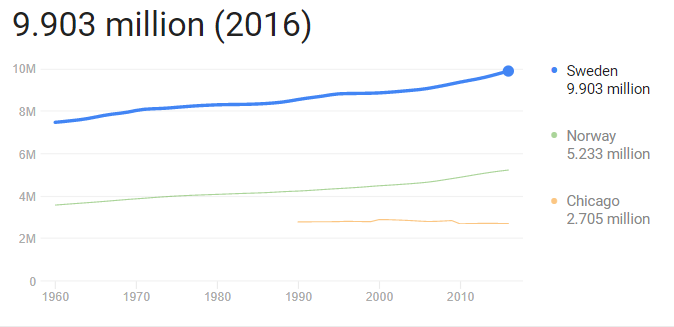
\includegraphics[width=1\linewidth]{swedPop}
\end{figure}
}
\only<2> {
\begin{figure}
	\centering
	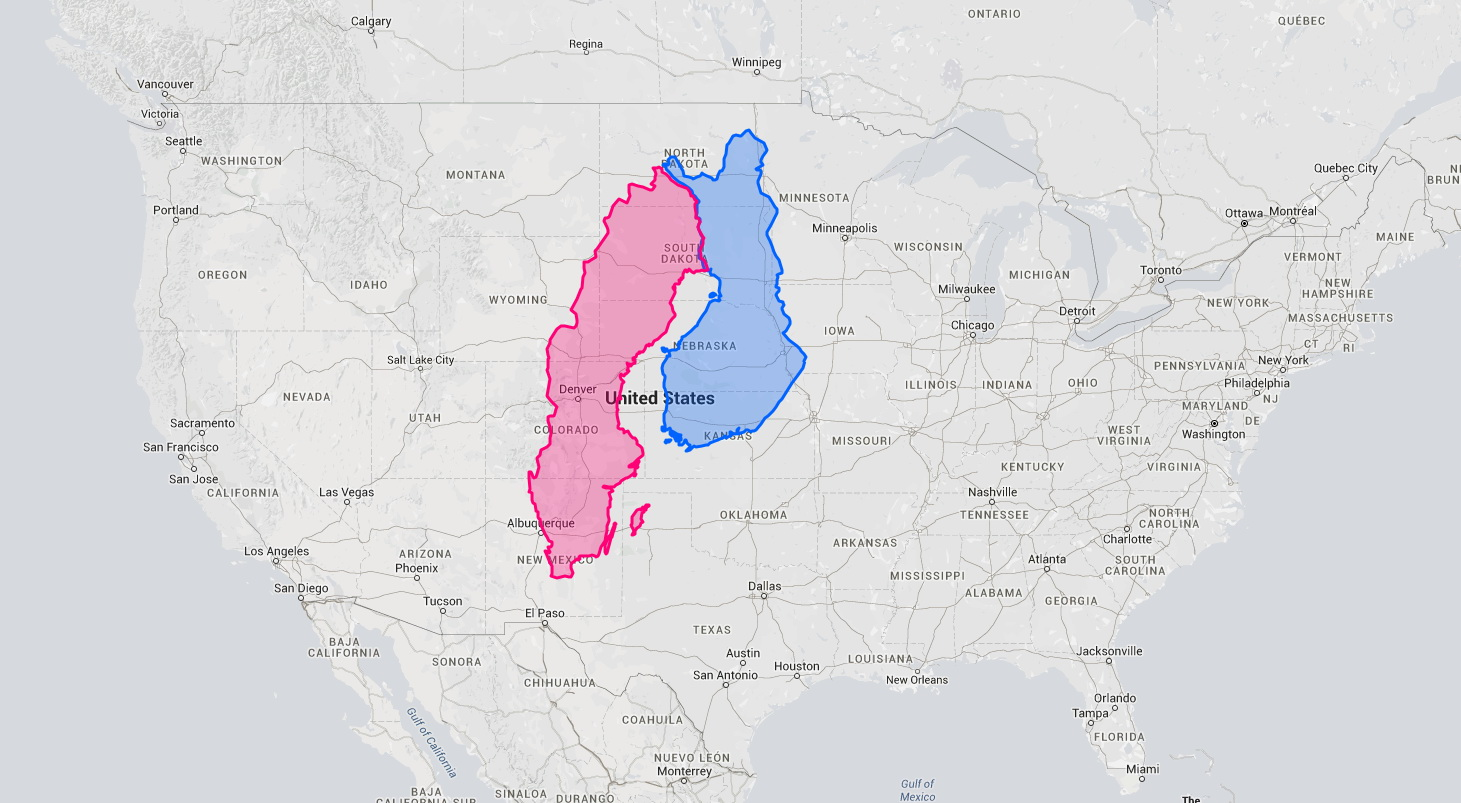
\includegraphics[width=1\linewidth]{swedenusa}
\end{figure}
}
\end{frame}

\begin{frame}{Introduction}

\onslide<2->{Sweden has a \alert{serious} problem. A problem with school fires.} \onslide<3->{Every single day, an average of \alert{one to two} schools are set ablaze.}
\begin{columns}
\column{0.5\textwidth}
\begin{figure}
\centering
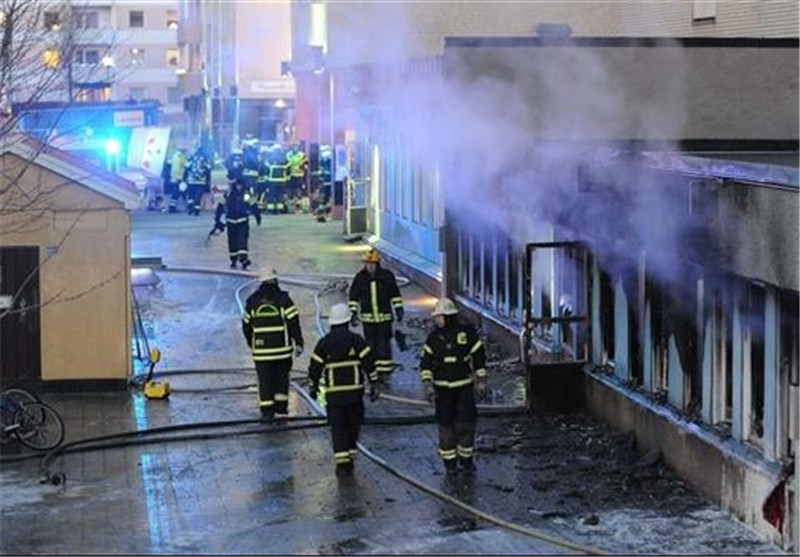
\includegraphics[width=1\linewidth]{fire1}
\end{figure}
\column{0.5\textwidth}
\begin{figure}
\centering
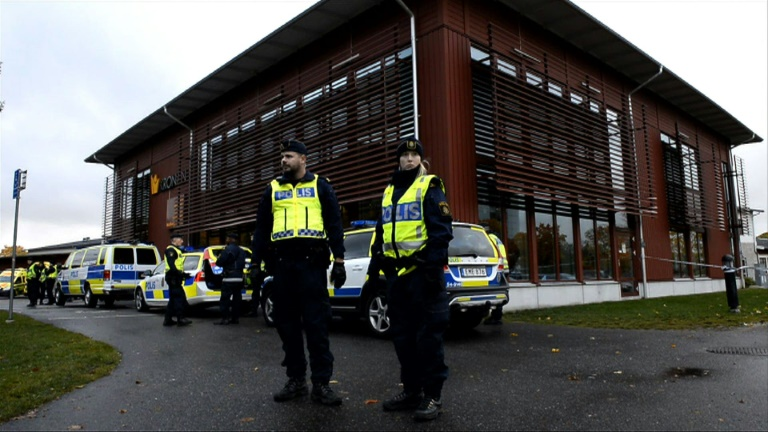
\includegraphics[width=1\linewidth]{fire2}
\end{figure}
\end{columns}

\end{frame}

\begin{frame}{By the numbers}
\begin{figure}[H]
\centering
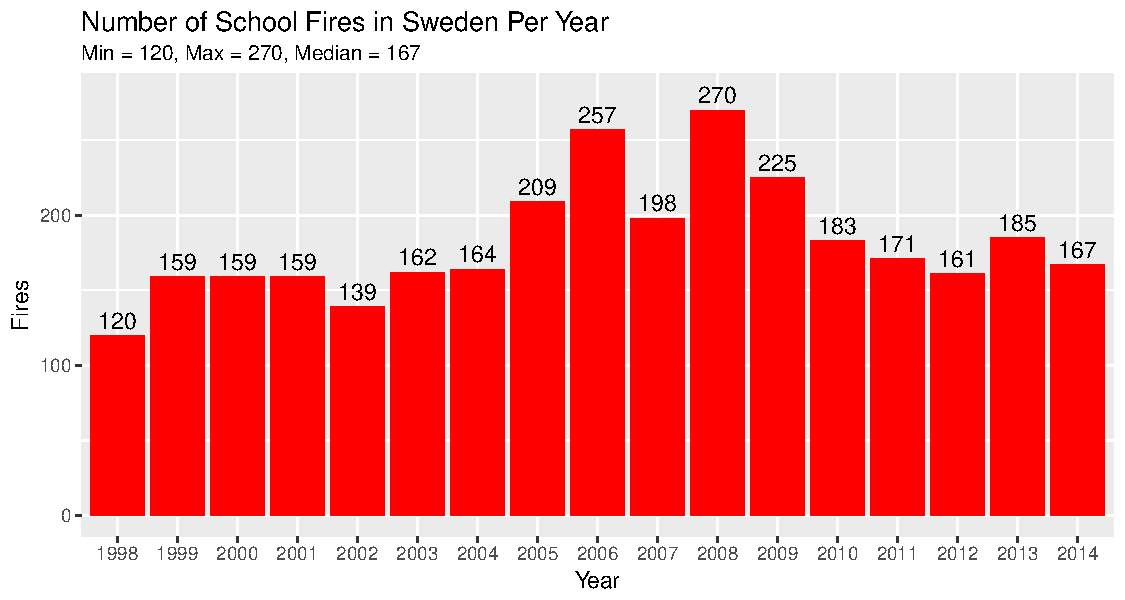
\includegraphics[width=1\linewidth]{FiresPerYear}
\end{figure}
\end{frame}


\begin{frame}{Geographic Heatmap}
\onslide*<1>{
\begin{figure}
\centering
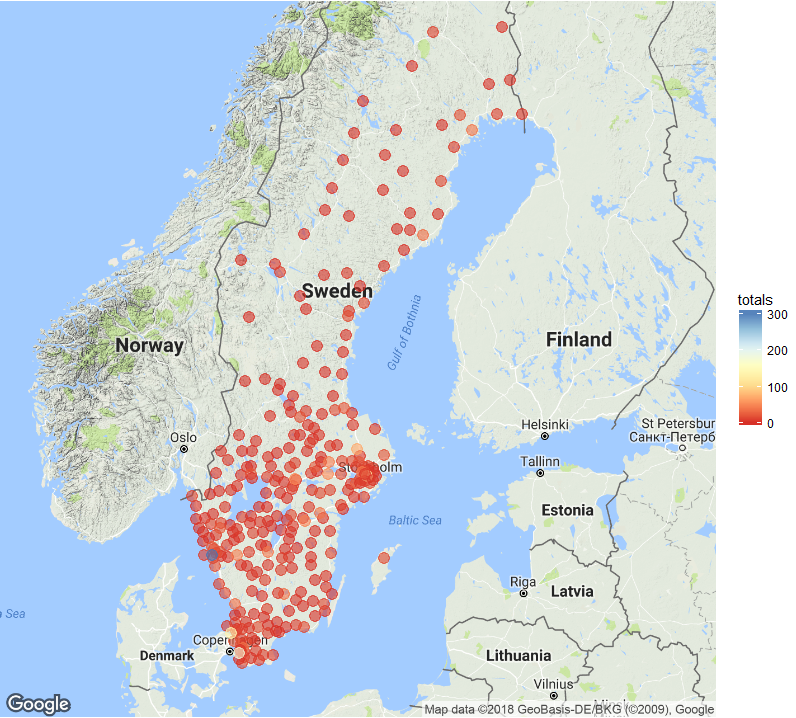
\includegraphics[width=0.7\linewidth]{Heatmap}
\end{figure}
}
\onslide*<2>{
\begin{figure}
\centering
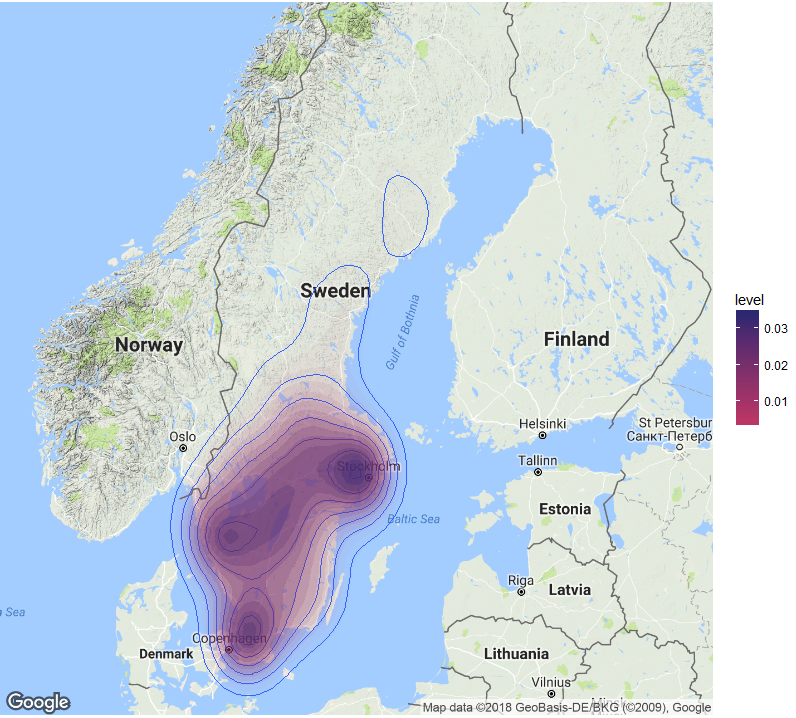
\includegraphics[width=0.7\linewidth]{HeatmapPoly}
\end{figure}
}
\onslide*<3>{
\begin{figure}
\centering
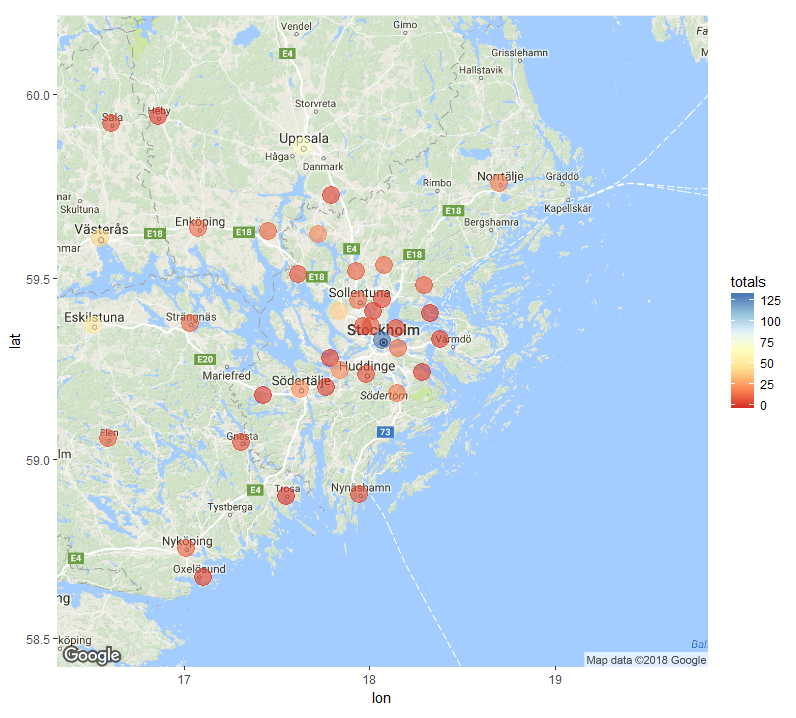
\includegraphics[width=0.7\linewidth]{HeatmapStockholm}
\end{figure}
}
\end{frame}



\begin{frame}{Introduction}
\begin{columns}[T]
\column{.5\textwidth}
\textbf{Background:} \vspace{0mm}
\begin{itemize}[<2->]
\item Sweden has a surprisingly large number of school fires for a small country ($<$ 10M inhabitants)
\item ``Almost every day between one and two school fires occur in Sweden. In most cases arson is the cause of the fire.'' 
\item The associated costs can be up to a billion SEK (around 120 million USD) per year.
\end{itemize}

\column{.5\textwidth}
\textbf{Aim:} \vspace{0.85mm}
\begin{itemize}[<3->]
\item To find out which properties and indicators of Swedish towns (municipalities, to be exact) might be related to a high frequency of school fires
\item Explore data to determine risk factors
\begin{itemize}
\item Geographic
\item Demographic
\item Cultural
\end{itemize}
\end{itemize}
\end{columns}
\end{frame}

\begin{frame}{The Costs...}
\begin{itemize}
\item The per-capita GDP of Sweden is $\approx \$51.6K$ USD
\item Thus school fires cost approximately 2,160 people their entire productivity for an entire year\ldots
\end{itemize}


\begin{figure}
\centering
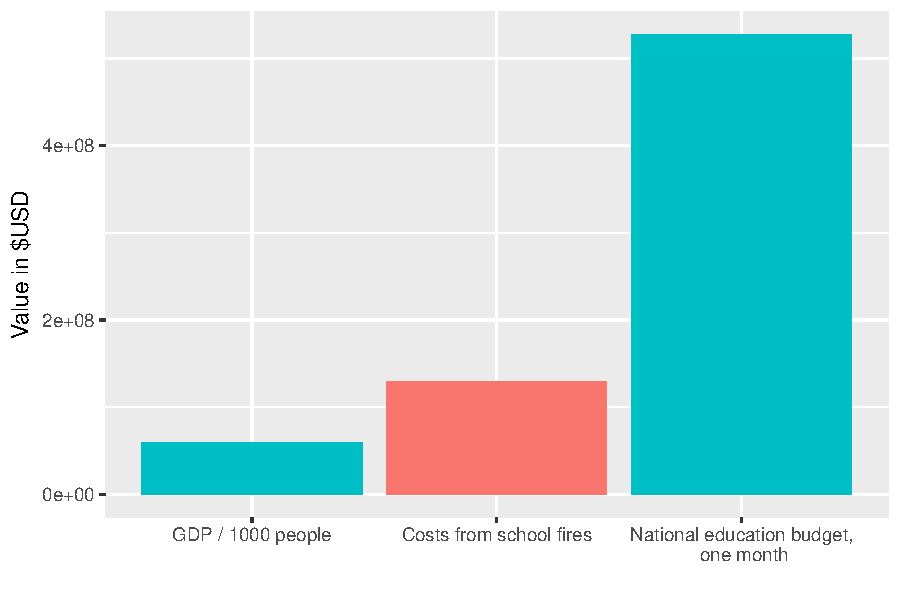
\includegraphics[width=.75\linewidth]{FireCosts}
\end{figure}
\end{frame}




\section{Data Set}
\begin{frame}{The Data Set}
The data set, indexed on a per-municipality basis, is quite rich. We have information on things as diverse as:
\begin{columns}[T]
\column{.5\textwidth}
\begin{itemize}
\item Income information
\item Unemployment information
\item Crime Rates
\item Foreign and domestic settlement rates
\item Satisfaction and psychological measures
\end{itemize}
\column{.5\textwidth}
\begin{itemize}
\item Per Capita Transportation Information
\begin{itemize}
\item Motorcycles
\item Autos
\item Snowmobiles
\item Tractors
\end{itemize}
\end{itemize}
\end{columns}
\end{frame}

\begin{frame}{The Data Set}

{\color{blue}{Goal:}} 
\begin{itemize}
\item Combine Demographic and Social Measures to identify high-risk areas and trends.
\item Predictive Analysis
\item Potential Cost Analysis
\end{itemize}

\vspace{1cm}
\pause

{\color{blue}{Potential Pitfalls:}}
\begin{itemize}
\item  Repeated Measurements
\item  Noisy Data
\item  Correlation of Neighbors
\end{itemize}
\end{frame}


\section{Discussion of Methods}
\begin{frame}{Discussion of Methods}
\begin{columns}

\column{.5\textwidth}
\textbf{Why Bayesian:} \vspace{0mm}
\begin{itemize}[<2->]
\item Multiple observations on a single municipality $\Rightarrow$ Errors exhibit correlation by municipality
\item Different years have different mean fire rates which need to be controlled
\item Each year, each municipality has a different population size
\item Potentially a correlation between years
\end{itemize}
\column{.5\textwidth}
\textbf{Contemplated Methods:} \vspace{0mm}
\begin{itemize}[<3>]
\item Linear Varying Effects Varying Intercepts Model
\item Linear Varying Effects Varying Intercepts Model with Correlation
\item Hierarchical Model with Time Series Components
\item Inspiration from \href{http://tharte.github.io/mbt/}{http://tharte.github.io/mbt/} and \href[]{http://www.ling.uni-potsdam.de/~vasishth/statistics/BayesLMMs.html}{http://www.ling.uni-potsdam.de/~vasishth/statistics/BayesLMMs.html}
\end{itemize}
\end{columns}
\end{frame}

\begin{frame}{Distribution of Work}
This project will require quite a lot of work to get off the ground. Included below are the current allocation of tasks for the project.
\begin{description}
\item[Andrei] Overall documentation and model validation
\item[Desmond] Pre-model exploration and processing
\item[Mark] Model Specification and Implementation in Base Stan
\item[Teerth] Data Visualization \& Post-model analysis
\end{description}
\end{frame}



%%%%%%%%%%%%%%%%%%%%%%%%%%%%%%%%%%%%%%%%%%%%%%%%%%%%%%%%%%%%%%%%%%%%%%%%%%%%%%%%
%                                                                              %
%                         Begin the model description                          %
%                                                                              %
%%%%%%%%%%%%%%%%%%%%%%%%%%%%%%%%%%%%%%%%%%%%%%%%%%%%%%%%%%%%%%%%%%%%%%%%%%%%%%%%

\newcommand{\munis}{\ensuremath{m}\xspace}
\newcommand{\years}{\ensuremath{y}\xspace}
\newcommand{\vars}[1]{\ensuremath{v_{#1}}\xspace}
\newcommand{\indic}[2]{\ensuremath{\mathbb{I}\left[#1 = #2\right]}\xspace}
\begin{frame}{Example Model Structure}
First some notation for the example linear model
\begin{itemize}
\item Let $M$ be the number of municipalities, indexed by \munis,
\item Let $Y$ be the number of years, indexed by \years,
\item Let $V$ be the number of explanatory variables, indexed by \vars{i},
\item Let $\beta$ denote a parameter and let subscripts denote indexing: $\beta_{(\munis)}$ is the  multiplier for a given municipality regardless of year or other  variables, and $\beta_{(\vars{i}, \years)}$ would be the multiplier of the $i^{th}$ variable during the $\years^{th}$ year
\item \indic{\Phi}{\phi} is an indicator function that is one when $\Phi = \phi$ and zero otherwise
\end{itemize}
\end{frame}

\begin{frame}[t]{Example Model Structure - Basic Linear Model}
Key detail of the model: All years and municipalities have the same mean - it is a linear function of the (scaled) predictors
\begin{align*}
\beta_0, \beta_{\vars{i}} &\sim P_{\bullet}(\bullet) \quad \text{[Choice of Priors]}\\
\lambda &= \beta_0 +  \sum_{i = 1}^{V} \beta_{\vars{i}} \vars{i}\\
Fires_{\munis, \years} &\sim Pois(\exp\left[\lambda\right])
\end{align*}
\onslide*<1>{
Some choices for $P_{\bullet}(\bullet)$:
\begin{description}
\item[Weakly Informative Prior] Let data drive the analysis with a weak prior
\item[Strong Normal Prior] Impose a strong normal prior around zero so that most coefficients will remain close to zero except for a select few
\item[Spike-and-Slab] Impose a mixture model for the coefficients in the form of a spike-and-slab prior to force most distributions to zero and let others vary
\end{description}
}
\onslide*<2>{
Some issues with the Basic Linear model:
\begin{description}
\item[Correlated Errors] We have multiple observations for each municipality, and thus the independence of the errors is violated
\item[Years clearly have different effects] The mean response for each year is clearly different from other years - see the histogram of effects at the beginning of the presentation
\item[Municipality Differences] Different Locations may respond differently to different predictors
\end{description}
}
\onslide*<3->{
Whats with the $\exp$ function wrapped around the mean variable?
\begin{itemize}
\item $\lambda$ takes its support on the positive reals, but we do not impose a positive definite solution on our linear equation form
\item We use the exponential to map $\mathbb{R}$ to $\mathbb{R}^{+}$ in a one-to-one fashion so that we do not need to impose domain restrictions in the model
\item<4> Truthfully, Stan just yelled at us for domain restrictions on a definite linear function... a lot \frownie
\end{itemize}

}

\end{frame}

\begin{frame}{Choices of Models}
We have a lot of directions to build off of this fixed effects model. We then take inspiration from Alice on this one:

\pause 
\vspace{1cm}
\begin{quote}
``Would you tell me, please, which way I ought to go from here?''\\
``That depends a good deal on where you want to get to.''\\
``I don't much care where –''\\
``Then it doesn't matter which way you go.''\\ 
-- Lewis Carroll, Alice in Wonderland
\end{quote}
%\pause 
%\begin{quote}
%	“Would you tell me, please, which way I ought to go from here?”\\
%	“That depends a good deal on where you want to get to,”\\
%	“I don’t much care where—”\\
%	“Then it doesn’t matter which way you go,” \\
%	“—so long as I get somewhere,” \\
%	“Oh, you’re sure to do that,” ... “if you only walk long enough.”\\ —Chapter 6, Pig and Pepper
%\end{quote}
\pause 
\vspace{1cm}

We choose to go down the mixed-effects modeling path and we will proceed with adding to our model to account for issues that arise in our data.
\end{frame}

\begin{frame}[t]{Example Model Structure - Mixed Effects Model}
Key detail of the model: Each year and municipality has a different mean that is incorporated - all variables are still included and each have the same overall effect regardless of municipality or year
\begin{align*}
\beta_0, \beta_{\vars{i}}, \beta_{(\munis)}, \beta_{(\years)} &\sim P_{\bullet}(\bullet) \quad \text{[Choice of Priors]}\\
\lambda_{\munis, \years} &= \beta_0 + \beta_{(\munis)} + \beta_{(\years)} + \sum\nolimits_{i = 1}^{V} \beta_{\vars{i}}\vars{i}\\
Fires_{\munis, \years} &\sim Pois(\exp\left[\lambda_{\munis, \years}\right])
\end{align*}
\onslide*<1>{
Some choices for $P_{\bullet}(\bullet)$ (as before):
\begin{itemize}
\item Weakly Informative Prior
\item Strong Normal Prior
\item Spike-and-Slab 
\end{itemize}
}
\onslide*<2>{
Some issues with the Mixed Effects Model
\begin{description}
\item[Yearly Trends] The effect of different variables could vary by year which could be a source of error
\item[Noise] With so many predictors, economic noise could really begin to be an issue if we do not introduce some regularizations
\end{description}
}
\end{frame}



\begin{frame}[t]{Example Model Structure - Mixed Effects Model 2 }
Key detail of the model: Each year and municipality has a different mean that is incorporated - all variables are still included and each has a different effect based on the year
\begin{align*}
\beta_0, \beta_{(\vars{i}, \years)}, \beta_{(\munis)}, \beta_{(\years)} &\sim P_{\bullet}(\bullet) \quad \text{[Choice of Independent Priors]}\\
\lambda_{\munis, \years} &= \beta_0 + \beta_{(\munis)} + \beta_{(\years)} + \sum\nolimits_{i = 1}^{V} \beta_{(\vars{i}, \years)} \vars{i}\\
Fires_{\munis, \years} &\sim Pois(\exp\left[\lambda_{\munis, \years}\right])
\end{align*}
\onslide*<1>{
Some choices for $P_{\bullet}(\bullet)$ (as before):
\begin{itemize}
\item Weakly Informative Prior
\item Strong Normal Prior
\item Spike-and-Slab 
\end{itemize}
}
\onslide*<2>{
Some issues with the Mixed Effects Model 2: 
\begin{description}
\item[Noise] With so many predictors, economic noise could really begin to be an issue if we do not introduce some regularizations
\item[Correlations] We still have not dealt with geographic correlations
\end{description}
}
\end{frame}

\begin{frame}[t]{Example Model Structure - Mixed Effects Model 3 }
\onslide*<1>{Key detail of the model: Each year and municipality has a different mean that is incorporated (and regularized by a hierarchical prior) - all variables are still included and each has a different effect based on the year.}
\begin{align*}
\beta_0 &\sim P_{\bullet}(\bullet) \quad \text{[Choice of Independent Priors]}\\
\beta_{(\vars{i}, \years)} &\sim N(\mu_{variable_i}, \sigma_{variable_i}) \quad \text{[Hierarchical Prior]}\\
\beta_{(\years)} &\sim N(\mu_{years}, \sigma_{years}) \quad \text{[Hierarchical Prior]}\\
\beta_{(\munis)} &\sim N(\mu_{muni}, \sigma_{muni}) \quad \text{[Hierarchical Prior]}\\
\lambda_{\munis, \years} &= \beta_0 + \beta_{(\munis)} + \beta_{(\years)} + \sum\nolimits_{i = 1}^{V} \beta_{(\vars{i}, \years)} \vars{i}\\
Fires_{\munis, \years} &\sim Pois(\exp\left[\lambda_{\munis, \years}\right])
\end{align*}
\onslide*<1>{
Shrinkage from the hierarchical prior prevents unconstrained departures from the group average effect making analysis more tractable. This model captures a great amount of variability.
}
\onslide*<2->{
Some issues with the Mixed Effects Model 3 
\begin{description}
\item[Lots of slope variables] We still have north of 1000 slope variables and some predictions may not be significantly different from zero\ldots \alert<3>{Perhaps take inspiration from the Hoff problem in Homework 4...}
\item[Correlations] We still have not dealt with geographic correlations
\end{description}
}
\end{frame}

\begin{frame}[t]{Example Model Structure - Mixed Effects Model 4 }
\onslide*<1>{Key detail of the model: Each year and municipality has a different mean that is incorporated (and regularized by a hierarchical prior) - all variables can now ``disappear'' based on their overall effect in the model and year}
\begin{align*}
\beta_0 &\sim P_{\bullet}(\bullet) \quad \text{[Choice of Independent Priors]}\\
\beta_{(\vars{i}, \years)} &\sim N(\mu_{variable_i}, \sigma_{variable_i}) \quad \text{[Hierarchical Prior]}\\
p_{\vars{i}} &\sim Beta\left(\nicefrac{1}{2}, \nicefrac{1}{2}\right)\\
\zeta_{\vars{i}} &\sim Bin(n = 1, p = p_{\vars{i}}) \quad \text{i.e.} \quad \zeta_{\vars{i}} \in [0,1]\\
\beta_{(\years)} &\sim N(\mu_{years}, \sigma_{years}) \quad \text{[Hierarchical Prior]}\\
\beta_{(\munis)} &\sim N(\mu_{muni}, \sigma_{muni}) \quad \text{[Hierarchical Prior]}\\
\lambda_{\munis, \years} &= \beta_0 + \beta_{(\munis)} + \beta_{(\years)} + \sum\nolimits_{i = 1}^{V} \beta_{(\vars{i}, \years)} \zeta_{\vars{i}} \vars{i}\\
Fires_{\munis, \years} &\sim Pois(\exp\left[\lambda_{\munis, \years}\right])
\end{align*}
\onslide*<2>{
The $p_{\vars{i}}$ variable can be interpreted to be the ``probability'' that a given variable is non-zero regardless of the year. This allows us to perform implicit feature selection and improve the fit. Bad variables will have low probability and good variables should have high probabilities. 
}
\onslide*<3>{
Some issues with the Mixed Effects Model 4
\begin{description}
\item[Correlations] We still have not dealt with geographic nor temporal correlations 
\end{description}
}

\end{frame}

\begin{frame}{Graphical Model}
\begin{figure}
	\centering
	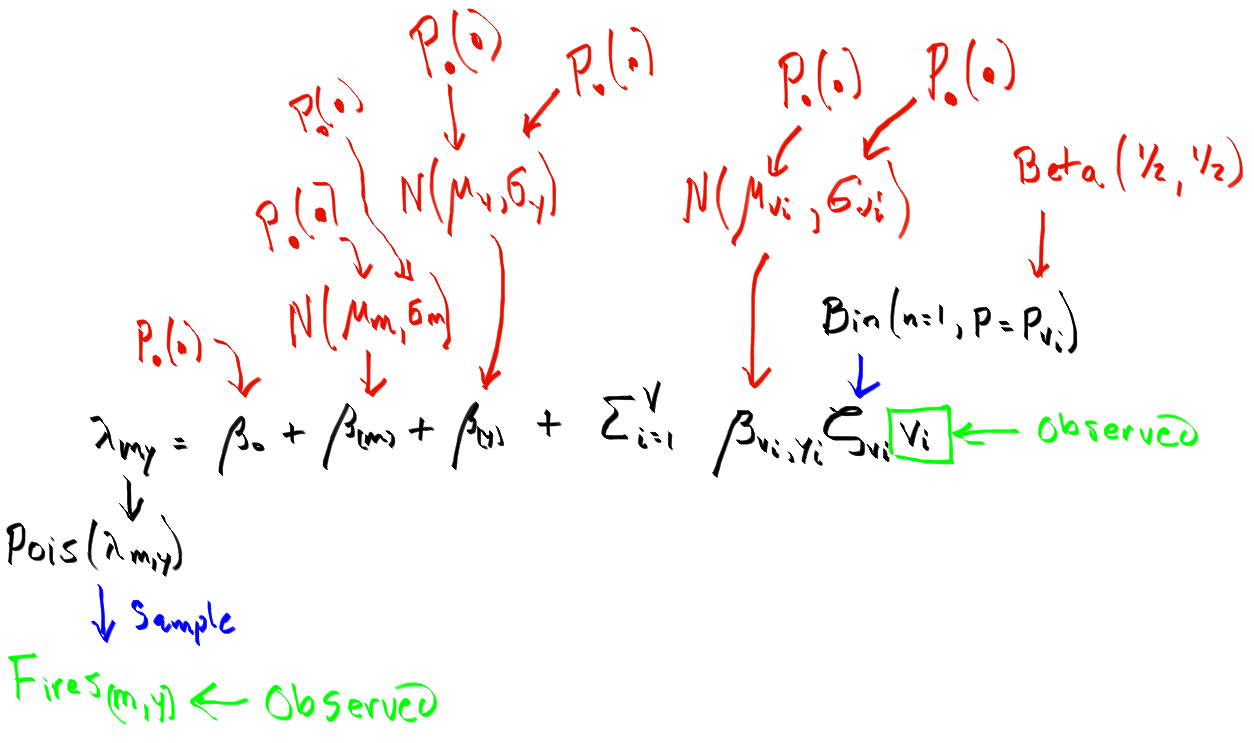
\includegraphics[width=0.90\linewidth]{Hierarchial_Model_Drawing}
	\caption{Let $P_{\bullet}(\bullet)$ be a (currently unspecified) modeling decision for a prior distribution. Red Denotes Priors, Green is Observed Data, and Black denotes structural forms}
	\label{fig:Hierarchicalmodeldrawing}
\end{figure}
\end{frame}

\begin{frame}[t]{The King Once Said}
Some issues with the Mixed Effects Model 4
\begin{description}
\item[Correlations] We still have not dealt with geographic nor temporal correlations  
\end{description}

\pause 

\vspace{1cm}
\begin{quote}
``Begin at the beginning,'' the King said, very gravely, ``and go on till you come to the end: then stop.'' \\
-- Lewis Carroll, Alice in Wonderland
\end{quote}	
\vspace{1cm}

\pause 


It is here that we have decided to end our journey down the modeling ``rabbit-hole'' and ``come up for air''. If our model is not able to sufficiently capture the complexity of the interactions, we will choose to incorporate temporal correlation and maybe spacial correlation. Until then, we chose to not complicate the model further.

\end{frame}

%\begin{frame}{Example Model Structure}
%\begin{align}
%	Fires_{(\years, \munis)} &\sim Pois\left(\lambda_{(\years, \munis)}\right)\\
%	\lambda_{(\years, \munis)} &= \beta_0 + \beta_{(\munis)} + \beta_{\years} + \sum\limits_{i = 1}^{V} \beta_{\vars{i}, \years}
%\end{align}
%\missingfigure{Under Construction}
%
%\end{frame}

%\begin{frame}
%	\begin{figure}
%	\centering
%	\begin{forest}
%		[$\lambda_y$ [$\mu_{Sweden_y}$ 
%		[$\mu_{m_{1,y}}$] 
%		[ $\cdots$]
%		[$\mu_{m_{k,y}}$ ]
%		][$\mu_{E_1}$ 
%		[$\mu_{E_{1,y},m_1}$] 
%		[ $\cdots$]
%		[$\mu_{E_{k,y},m_k}$ ]
%		][$\cdots$]]
%	\end{forest}
%\end{figure}
%\missingfigure{Under Construction}
%
%	
%\end{frame}





\section{Preliminary Findings}
\begin{frame}{Preliminary Findings - Model}
To get an initial sense of predictor-outcome relationships, we ran a preliminary model using the rstanarm package. This preliminary model uses total recent fires (from 2010-2014) as the outcome, does not include year/municipality-specific parameters, and uses 2-knot spline functions S of each included predictor.

\begin{align*}
Fires_{m} \sim Poisson(\lambda) \\
Fires_{m} = \beta_0 + \sum_{i=1}^V \beta_i S(v_i) \\
\beta_1,...,\beta_V \sim N(0,1)
\end{align*}
\end{frame}

\begin{frame}{Preliminary Findings - Parameters}

\begin{figure}
\centering
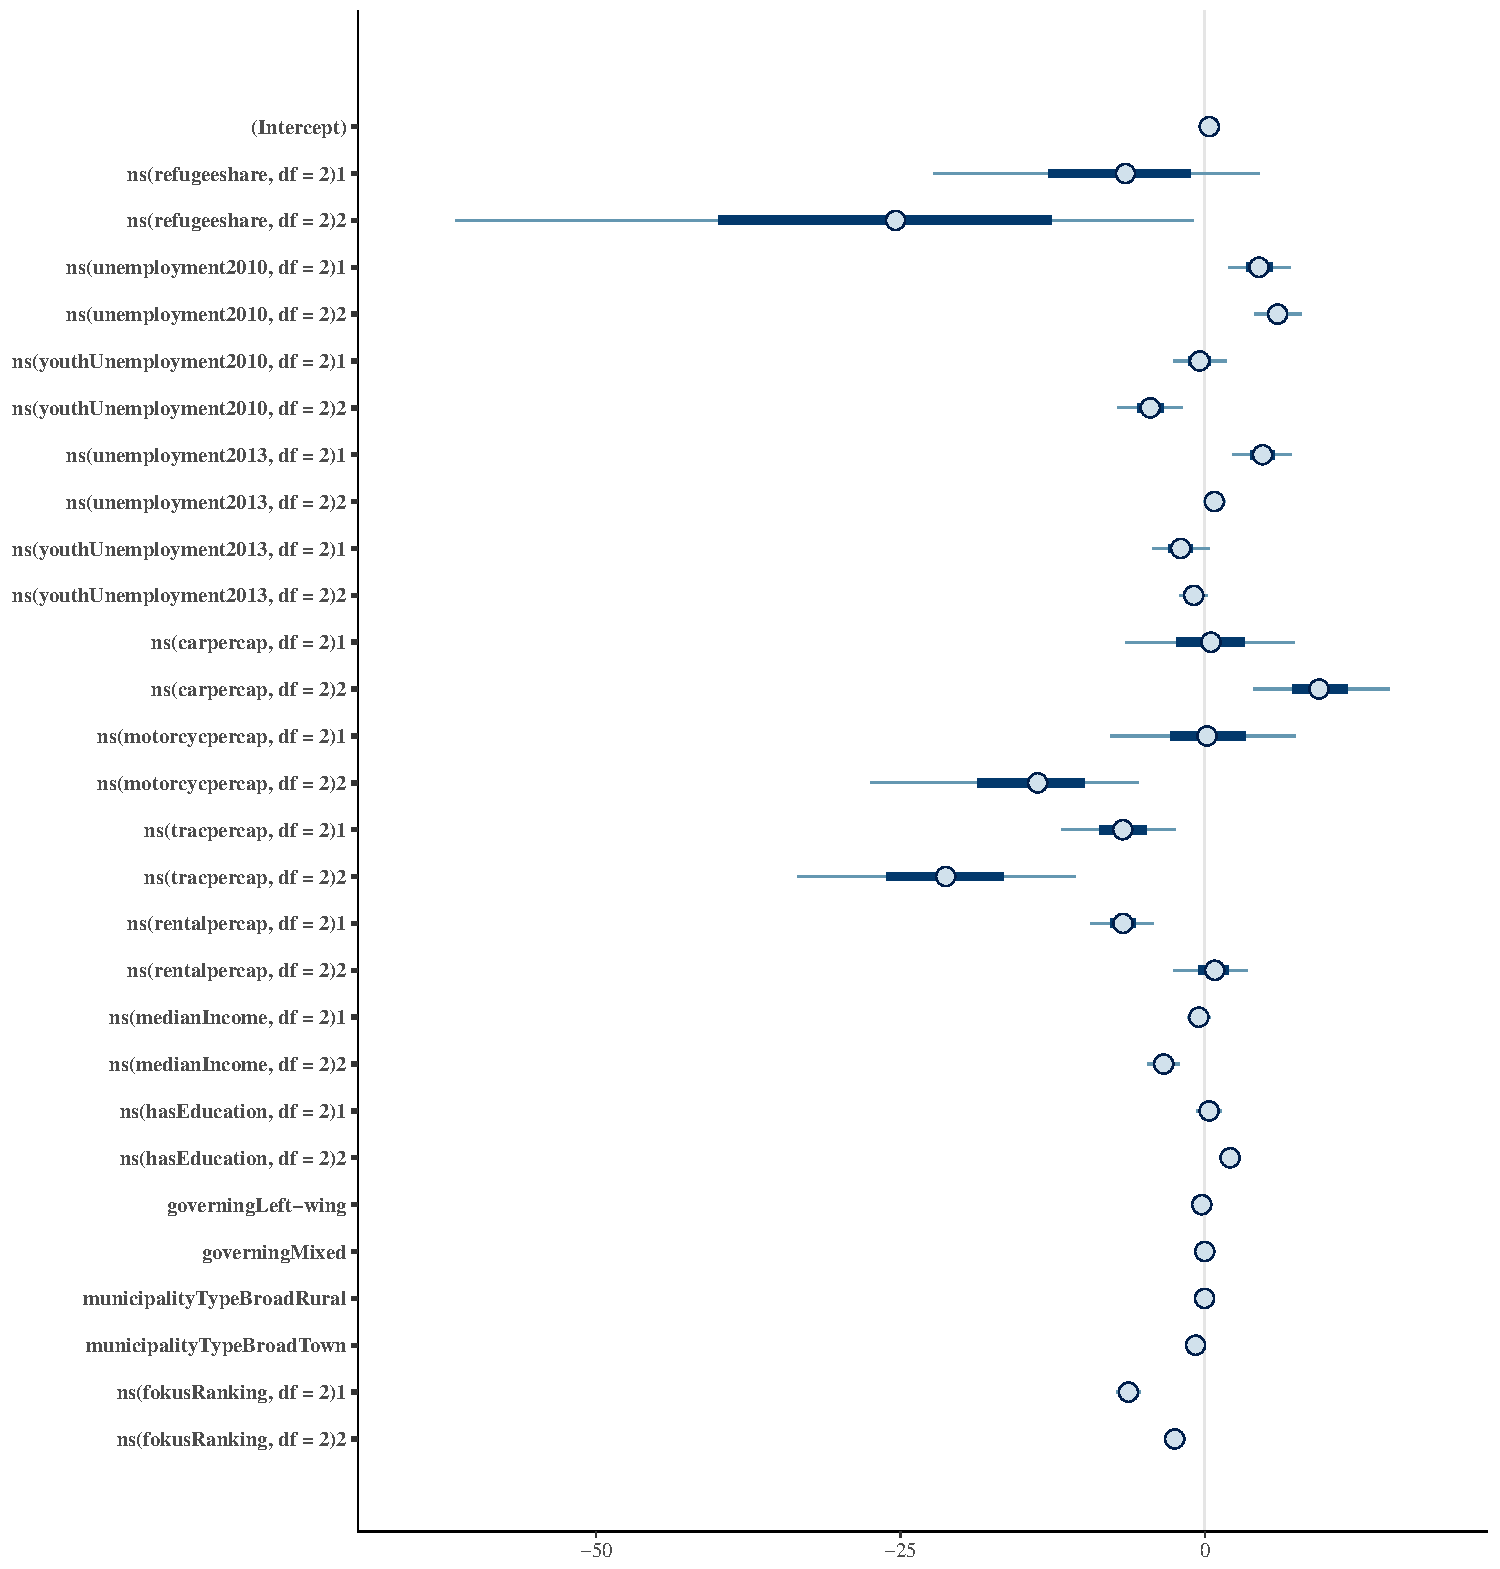
\includegraphics[width=.6\linewidth,height=8cm]{parameterintervals.pdf}
\end{figure}

\end{frame}




\end{document}





